\documentclass{article}

\usepackage[utf8]{inputenc}
\usepackage[italian]{babel}
\usepackage[T1]{fontenc}

\usepackage[a4paper,top=2cm,bottom=2cm,left=3cm,right=3cm]{geometry}
\usepackage{hyperref, xr, amsmath, amssymb, graphicx, mathtools, xcolor, enumitem, verbatim, todonotes, csquotes, subcaption, fancyhdr, lastpage, cancel, xspace, float, caption, prettyref}
\usepackage[most]{tcolorbox}

\externaldocument[D1-]{../D1/out/ObiettiviDelProgetto}
\newrefformat{D1-ob}{\color{blue}D1 \ref{#1}\color{black}}

\externaldocument[D1-]{../D1/out/RequisitiFunzionali}
\newrefformat{D1-rf}{\color{blue}D1 \ref{#1}\color{black}}

\externaldocument[D1-]{../D1/out/RequisitiNonFunzionali}
\newrefformat{D1-rnf}{\color{blue}D1 \ref{#1}\color{black}}

\externaldocument[D1-]{../D1/out/RequisitiFrontEnd}
\newrefformat{D1-fe}{\color{blue}D1 \ref{#1}\color{black}}

\externaldocument[D1-]{../D1/out/RequisitiBackEnd}
\newrefformat{D1-be}{\color{blue}D1 \ref{#1}\color{black}}
\title{Report Finale}
\author{Gruppo T56}
\date{A.A. 2022-2023}

%\setlength\parindent{0pt}

\setcounter{tocdepth}{5}
\setcounter{secnumdepth}{5}

\lhead{\textbf{Document: }Report Finale}
\rhead{\textbf{Revision: }0.1}
\cfoot{\thepage /\pageref{LastPage}}

\hypersetup{
    colorlinks=true,
    linkcolor=blue,
    urlcolor=blue,
    pdftitle={Report Finale - Gruppo T56},
}

\pagestyle{fancy}
\newcommand{\nome}[0]{Life Planner\xspace}

\begin{document}

\begin{titlepage}
    \begin{figure}[!htb]
        \minipage{0.5\textwidth}
        \includegraphics[width=0.7\textwidth]{img/logo_unitn.png}
        \endminipage
        \hfill
        \minipage{0.5\textwidth}
        \begin{flushright}
            \Large
            Dipartimento d'Ingegneria e Scienze dell'informazione
        \end{flushright}
        \endminipage
        \hfill
    \end{figure}

    \vspace{6cm}

    \large
    \textbf{Progetto:}
    \begin{center}
        \Huge
        \color{blue}
        \textbf{Life planner}
    \end{center}

    \vspace{1cm}

    \textbf{Titolo del documento:}
    \begin{center}
        \huge
        \color{blue}
        \textbf{Documento di progetto}\\
        \textbf{(Obiettivi e Requisiti)}
    \end{center}


    
\end{titlepage}
\pagebreak

\tableofcontents
\pagebreak

\section*{Scopo del documento}
\addcontentsline{toc}{section}{Scopo del documento}
Lo scopo di questo documento è presentare gli obiettivi, i requisiti e i design Front-End e Back-End del progetto \nome ideato da Gabriele Lacchin, Denis Lucietto ed Emanuele Zini.\\
Il seguente documento presenta:
\begin{itemize}
    \item \hyperref[secD1:ObiettiviDelProgetto]{gli obiettivi del sistema};
    \item \hyperref[secD1:RequisitiFunzionali]{i requisiti funzionali};
    \item \hyperref[secD1:RequisitiNonFunzionali]{i requisti non funzionali};
    \item \hyperref[secD1:RequisitiFrontEnd]{design Front-End};
    \item \hyperref[secD1:RequisitiBackEnd]{design Back-End}.
\end{itemize}
\section{Obiettivi del progetto}
Il progetto ha come obiettivo la realizzazione di un life planner automatizzato.\\
Il sito si pone come un sistema automatizzato di programmazione del tempo in base agli impegni che si inseriscono, avendo la possibilità d'imporre delle preferenze per la disposizione delle attività da svolgere.\\
La funzione principale del life planner è la facilitazione del processo di programmazione del proprio tempo.

\vspace{0.5cm}

Nello specifico questa applicazione permette di:
\begin{itemize}
    \item Compilare tramite un pop-up un impegno da aggiungere al proprio calendario.
    \item Poter applicare delle restrizioni riguardo a quando l'impegno può esser posto.
    \item Una volta creato un impegno viene automaticamente impostata una data a meno di restrizioni.
    \item Avere la possibilità di gestire anche routine e impegni ripetuti.
    \item Impostare priorità impegno.
    \item Impostare preferenze su quanto dormire.
    \item Notifiche per ciascuno impegno.
    \item Ogni evento ha la possibilità d'impostare notifiche personalizzate
    \item Integrare con Google calendario
    \item Infografiche sull'uso del tempo
    \item In caso di ritardi con un attività in automatico riorganizza le altre attività
\end{itemize}

\todo{Finire Obiettivi}

\section{Requisiti funzionali}
\label{sec:RequisitiFunzionali}

Nel seguente capitolo verranno presentati i requisiti funzionali (RF) del sistema con la motivazione della loro presenza e legame con gli obiettivi sopra citati.
\begin {listaPersonale}{RF}
\elemento[ACCESSO E REGISTRAZIONE AL SITO]{rf:1} 
Il sistema deve permettere all'utente di avere 3 livelli di accesso:
\begin{itemize}
	\item utente autenticato-standard(\ref{ob:1});
    \item utente non autenticato (\ref{ob:1}); 
    \item utente autenticato-premium (\ref{ob:6});
\end{itemize}
Il sistema deve permettere all'utente di registrarsi sul sito (\ref{ob:1}) in qualsiasi momento esso voglia e inoltre deve permettere di abbonarsi al servizio premium, con un account preesistente o anche durante la fase di registrazione.\\
Ad ogni modo il sistema deve rendere disponibile all'utente di utilizzare il sito anche come utente non autenticato in versione demo(\ref{rf:3}). 


\begin {listaPersonale2}{RF}
\elemento[METODI AUTENTICAZIONE]{rf:1:1}
L'autenticazione può essere fatta con email e password o con servizi di terze parti, più nello specifico con Google, Facebook, LinkedIn, Twitter e Apple (\ref{ob:1}).
\end {listaPersonale2}


\elemento[UTENTE AUTENTICATO-STANDARD]{rf:2}
Un utente autenticato standard è un utente registrato che ha effettuato il login e che usufruisce delle funzionalità base della piattaforma.

\begin {listaPersonale2}{RF}
\elemento[FUNZIONALITA’]{rf:2:1}
Il sistema offrirà agli utenti con account autenticato-standard tutti i servizi sottoelencati, eccetto quelli descritti nella sezione utente autenticato-premium (\ref{rf:2.2}), con le limitazioni elencate in \ref{rf:2.2.2}.

\elemento[UTENTE AUTENTICATO-PREMIUM]{rf:2.2}
L’utente avrà la possibilità anche di accedere ad un maggior numero di funzionalità della piattaforma grazie alla sottoscrizione di un abbonamento mediante un pagamento mensile.
Inoltre il pagamento degli utenti premium contribuirà alla sostenibilità economica del sito(\ref{ob:6}).

\begin {listaPersonale3}{RF}
\elemento[PAGAMENTO]{rf:2.2.1}
Il sistema offrirà la possibilità all’utente di pagare l’abbonamento con un servizio esterno, ovvero PayPal e/o Stripe. (\ref{ob:6})


\elemento[FUNZIONALITA’ AGGIUNTIVE(\ref{ob:6})]{rf:2.2.2}
Grazie all’account premium, il sistema permetterà di accedere alle funzionalità standard e a dei servizi aggiuntivi:
\begin{itemize}
    \item poter avere un numero illimitato di calendari personali in base allo loro scopo: gli utenti non premium potranno avere solo 5 calendari personali.
    \item poter avere un numero illimitato di calendari condivisi: gli utenti standard potranno averne 3.
\end{itemize}


\end {listaPersonale3}
\end {listaPersonale2}

\elemento[UTENTE NON AUTENTICATO]{RF:3} 
Nel caso di un utente non autenticato (\ref{ob:1}), il sistema permetterà di effettuare l’accesso e/o registrazione nelle modalità descritte in \ref{rf:1}. Nel caso l’utente non volesse registrarsi o accedere, il sito darà la possibilità di usufruire delle funzionalità in versione demo.

\begin{listaPersonale2}{RF}
    \elemento{DEMO}{rf:3.1}
    L'utente non autenticato avrà la possibilità di utilizzare il sito senza che le modifiche
    fatte vengano salvate sui server delle piattaforma; nel caso in cui l'utente si registrasse sul sito, verranno caricate e rese disponibili su più dispositivi.

\begin{listaPersonale3}{RF}
	\elemento[FUNZIONALITÀ MANCANTI]{rf:3.1.1}
    L’utente non autenticato non avrà a disposizione diverse funzionalità tra cui \ref{rf:4}, \ref{rf:8}, \ref{rf:10}, \ref{rf:11}.
\end{listaPersonale3}

\end{listaPersonale2}

RF4 CONDIVISIONE DEL CALENDARIO 
Il sistema darà la possibilità di condividere il proprio calendario su più dispositivi (\ref{ob:8}).

RF4.1 INTERAZIONE DI CALENDARI CON ALTRE PERSONE
Il sistema deve offrire la possibilità agli utenti autenticati di interagire tra loro 
mediante la condivisione e integrazione dei loro calendari (\ref{ob:8}). 
Grazie alla condivisione e integrazione dei calendari tra gli utenti del sito, i clienti avranno la possibilità di programmare gli eventi in comune.

RF5 COMPILAZIONE EVENTO 
Il sistema deve dare la possibilità all'utente di aggiungere un evento al calendario mediante un pop-up (\ref{ob:2}). 
Nella compilazione dell’attività, il sistema deve permettere al cliente: 
	-RF5.1 di imporre restrizioni, per esempio definire ora e giorno dell’attività da svolgere; 
	-RF5.2 impostare la priorità dell'impegno;
	-RF5.3 scrivere una descrizione e un titolo;
	-RF5.4 definire impegni di routine oppure impegni ripetuti su 
	più giorni. 
-RF5.5 L’utente avrà la possibilità di impostare le ore di sonno giorno per giorno oppure applicare le stesse ore per più giorni.

RF6 IMPOSTAZIONE IMPEGNO
Una volta compilato il pop-up di aggiunta impegno, il sistema deve inserire l'impegno nel calendario (\ref{ob:3}) seguendo le restrizioni e priorità inserite dall'utente a tempo di compilazione dell'evento (RF5).


RF7 NOTIFICHE
Il sistema deve inviare delle notifiche per ciascun impegno (\ref{ob:4}), fornendo la possibilità di 
personalizzarle, infatti nel pop-up di compilazione dell'evento (RF5) deve essere possibile: 
	-RF7.1: impostare quando ricevere tale notifica
	-RF7.2: definire il titolo della notifica: di default quest'ultimo sarà il titolo dell’evento.

RF8 INTERAZIONE CON SISTEMI DI TERZE PARTI
Il sito deve permettere all’utente di interagire con sistemi di terzi parti (\ref{ob:5}), ad esempio:

RF8.1 INTERAZIONE con GOOGLE CALENDAR
In quanto è un'applicazione molto diffusa tra gli utenti che utilizzano calendari,
il sistema deve rendere possibile all'utente di poter interagire eventi da Google Calendar. 
In particolare: 
	-RF8.1.1 si potranno importare eventi da Google Calendar, e questi, quando saranno aggiunti, saranno importati nel calendario personale seguendo le stesse regole per gli impegni aggiunti direttamente dal sito (si veda RF5).
	-RF8.1.2 si potranno esportare gli eventi dai diversi calendari personali a Google Calendar.

RF8.2 INTERAZIONE con Google Maps
Il sistema darà la possibilità all’utente di aggiungere il luogo dove si svolgerà l’impegno.


RF9 INFORMAZIONI sull’USO del TEMPO
Il sito deve presentare delle infografiche sull'uso tempo. L'utente, così, potrà
visualizzare dei grafici esemplificativi su come viene speso il proprio tempo. 
(\ref{ob:12})

RF10 RIORGANIZZAZIONE DI ATTIVITA' 
Il sistema deve riorganizzare automaticamente il calendario in caso di ritardi (\ref{ob:3}). Sarà data la possibilità all'utente di notificare il sistema di ritardi e il sito dovrà ripianificare il calendario, sempre secondo le regole descritte nel RF6. 

RF11 RESOCONTO GIORNATA
Il sistema, a fine giornata, deve presentare un resoconto (\ref{ob:7}), dove l'utente potrà
comunicare le attività fatte e non, in modo tale da dare la possibilità al sistema di 
ricalcolare eventuali modifiche in base agli impegni non conclusi sempre secondo le modalità citate in RF6.

RF12 FILTRO IMPEGNI 
Il sito offrirà la possibilità di poter visualizzare gli impegni dato un specifico filtro(\ref{ob:10}) definito dall’utente secondo alcuni criteri: 
RF12.1 Titolo evento con corrispondenza totale o parziale.
RF12.2 Data evento.
RF12.3 Priorità evento.
RF12.4 Persone incluse nell’evento.

\end{listaPersonale}


\section{Requisiti non funzionali}
\label{secD1:RequisitiNonFunzionali}

\begin{listaPersonale}{RNF}
      \elemento[PRIVACY]{rnf:Privacy} L'applicazione deve essere progettata e realizzata in ottemperanza del Regolamento per la protezione dei dati (GDPR) dell'Unione Europa entrata in vigore nel 2016 (\ref{ob:SicurezzaPrivacyCookie}). In specifico il sito dovrà adempiere:
      \begin{listaPersonale2}[RNF]{}
            \elemento{rnf:TrattamentoLecitoPrivacy} \href{https://eur-lex.europa.eu/legal-content/IT/TXT/?uri=uriserv:OJ.L_.2016.119.01.0001.01.ITA&toc=OJ:L:2016:119:TOC#d1e1898-1-1}{Capo 2, Articolo 6} trattamento lecito dei dati personali; poiché i dati personali sono necessari per il legittimo interesse di utilizzo del sito, il consenso sarà richiesto solo per alcune funzionalità (Es. \ref{rf:CondivisioneCalendario}). In caso il consenso non venisse dato l'utente non autenticato non potrà avere accesso ad alcune funzionalità della piattaforma.
            \begin{listaPersonale3}[RNF]{}
                  \elemento{rnf:ObblighiDiLeggePrivacy} In caso di un utente premium il sistema richiederà ulteriori dati, tra cui quelli di fatturazione, i quali saranno obbligatori per adempiere agli obblighi di legge.
            \end{listaPersonale3}

            \elemento{rnf:InformativaFinalitaPrivacy} Creare un'informativa sulle finalità e modalità dei trattamenti: il contenuto dell'informativa dovrà presentare le istruzioni date nel \href{https://eur-lex.europa.eu/legal-content/IT/TXT/?uri=uriserv:OJ.L_.2016.119.01.0001.01.ITA&toc=OJ:L:2016:119:TOC#d1e2261-1-1}{Capo 3, Sezione 2, Articolo 13} del GDPR, ovvero:
            \begin{listaPersonale3}[RNF]{}
                  \elemento{rnf:CategoriaDatiInformativaPrivacy} categoria di dati raccolti;
                  \elemento{rnf:FinalitaInformativaPrivacy} finalità del trattamento;
                  \elemento{rnf:PeriodoConservazioneInformativaPrivacy} periodo di conservazione;
            \end{listaPersonale3}

            \elemento{rnf:PresentazionePrivacy} a dei requisiti di presentazione, ovvero l'informativa deve essere chiara, concisa, facilmente accessibile e comprensibile;

            \elemento{rnf:DirittiPrivacy} al riconoscimento di alcuni diritti, ovvero:
            \begin{listaPersonale3}[RNF]{}
                  \elemento{rnf:DirittoAccessoDatiPrivacy} diritto di accesso ai dati da parte dell'utente standard (\href{https://eur-lex.europa.eu/legal-content/IT/TXT/?uri=uriserv:OJ.L_.2016.119.01.0001.01.ITA&toc=OJ:L:2016:119:TOC#d1e2520-1-1}{Capo 3, Sezione 2, Articolo 15});
                  \elemento{rnf:DirittoRettificaPrivacy} diritto di rettifica (\href{https://eur-lex.europa.eu/legal-content/IT/TXT/?uri=uriserv:OJ.L_.2016.119.01.0001.01.ITA&toc=OJ:L:2016:119:TOC#d1e2606-1-1}{Cap 3, Sezione 3, Articolo 16});
                  \elemento{rnf:DirittoOblioPrivacy} diritto all'oblio/cancellazione (\href{https://eur-lex.europa.eu/legal-content/IT/TXT/?uri=uriserv:OJ.L_.2016.119.01.0001.01.ITA&toc=OJ:L:2016:119:TOC#d1e2613-1-1}{Cap 3, Sezione 3, Articolo 17});
                  \elemento{rnf:DirittoOpposizionePrivacy} diritto di opposizione (\href{https://eur-lex.europa.eu/legal-content/IT/TXT/?uri=uriserv:OJ.L_.2016.119.01.0001.01.ITA&toc=OJ:L:2016:119:TOC#d1e2810-1-1}{Cap 3, Sezione 4, Articolo 21});
            \end{listaPersonale3}

            \elemento{rnf:EsercizioDeiDirittiPrivacy} alla resa facile e gratuita nell'esercizio dei propri diritti (\href{https://eur-lex.europa.eu/legal-content/IT/TXT/?uri=uriserv:OJ.L_.2016.119.01.0001.01.ITA&toc=OJ:L:2016:119:TOC#d1e2189-1-1}{Capo 3, Sezione 1, Articolo 12, Comma 2});
            \elemento{rnf:ViolazioneSistemaPrivacy} a informare gli utenti in caso di violazione (\href{https://eur-lex.europa.eu/legal-content/IT/TXT/?uri=uriserv:OJ.L_.2016.119.01.0001.01.ITA&toc=OJ:L:2016:119:TOC#d1e3497-1-1}{Capo 4, Sezione 2, Articolo 34});
      \end{listaPersonale2}


      \elemento[SICUREZZA]{rnf:Sicurezza} Il sito di rete deve essere progettato e realizzato per garantire la sicurezza dei dati (\ref{ob:SicurezzaPrivacyCookie}) adottando pratiche e metodologie nella fase di trasmissione di dati tramite rete Internet, ad esempio il sito dovrà provvedere a:
      \begin{listaPersonale2}[RNF]{}
            \elemento{rnf:SicurezzaPassword} avere, come primo livello di sicurezza, una password ed email decisa obbligatoriamente dagli utenti in fase di registrazione. La password deve seguire degli standard, ovvero avere almeno:
            \begin{itemize}
                  \item otto caratteri;
                  \item una lettera maiuscola;
                  \item una lettera minuscola;
                  \item un simbolo;
                  \item un numero.
            \end{itemize}
            \elemento{rnf:AttacchiSicurezza} mantenere privati i dati degli utenti ed evitare attacchi di rete tipo "sniffing" o "man in the middle";
            \elemento{rnf:OrigineDatiSicurezza} applicare politiche sull'origine dei dati;
            \elemento{rnf:XSSSicurezza} assicurare che non possano essere effettuati attacchi XSS;
            \elemento{rnf:DDOSSicurezza} alla protezione dei server da attacchi DDOS.
      \end{listaPersonale2}

      \elemento[SCALABILITÀ]{rnf:Scalabilita} L'applicazione deve garantire l'elaborazione di un numero crescente di utenti in modo tale da offrire tutte le sue funzionalità indipendentemente dal numero di utenti connessi (\ref{ob:Scalabilita}).

      \elemento[AFFIDABILITÀ]{rnf:Affidabilita} Il sito deve garantire il funzionamento delle funzionalità che ci si aspetta vengano eseguite quando viene fatta una determinata azione da parte dell'utente standard (\ref{ob:Caratteristiche}), per questo motivo:
      \begin{listaPersonale2}[RNF]{}
            \elemento{rnf:ConfermaServerAffidabilita} un'azione non è definita completata fintanto che il server non confermi l'avvenuto successo dell'azione richiesta;
            \elemento{rnf:GestioneEccezioniAffidabilita} tutte le eccezioni devono essere gestite con errori appropriati;
            \elemento{rnf:ResilienteFallimentoAffidabilita} la piattaforma deve essere progettata in modo tale di essere resiliente in caso di fallimento di uno dei suoi componenti.
      \end{listaPersonale2}

      \elemento[PRESTAZIONI]{rnf:Prestazioni} Il sito dovrà presentare almeno un punteggio di 85\% durante nella valutazione delle prestazioni (\ref{ob:Caratteristiche}) mediante l'utilizzo dello strumento “lighthouse” di Google Chrome.

      \elemento[COMPATIBILITÀ]{rnf:Compatibilita} Il sito deve essere compatibile (\ref{ob:Caratteristiche}) con i browser Chromium based, Firefox e Safari di edizione 2022.

      \elemento[WEB APP]{rnf:WebApp} La piattaforma dovrà rendere disponibile all'utente non autenticato una web app (\ref{ob:WebApp}) per aumentare le funzionalità offerte.

      \elemento[INTEROPERABILITÀ]{rnf:Interoperabilita} Il sistema deve poter operare con sistemi esterni (\ref{ob:ServiziTerzeParti}), che prestano delle funzionalità aggiuntive nella piattaforma, non implementate direttamente dal sito. In modo specifico i sistemi esterni presenti dovranno essere:
      \begin{listaPersonale2}[RNF]{}
            \elemento{rnf:MappeInteroperabilita} sistemi di mappe, vale a dire Google Maps e OpenStreetMap;
            \elemento{rnf:PagamentoInteroperabilita} sistemi di pagamento, vale a dire PayPal e Stripe;
            \elemento{rnf:AutenticazioneInteroperabilita} sistemi di autenticazione, vale a dire Auth0; % prima questi servizi di terze parti non erano specificati, non so perché. GL
            \elemento{rnf:GoogleCalendarInteroperabilita} Google Calendar.
      \end{listaPersonale2}

      \elemento[PORTABILITÀ]{rnf:Portabilita} Il sistema deve essere capace di adattarsi (\ref{ob:ServiziTerzeParti}) a diversi dispositivi le cui dimensioni possono essere variabili.

      \elemento[LINGUA DI SISTEMA]{rnf:Lingua} Il sito deve essere fornito in lingua italiana (\ref{ob:Caratteristiche}).

      \elemento[COOKIE]{rnf:Cookie} Il sito fa utilizzo di cookie (\ref{ob:SicurezzaPrivacyCookie}) per memorizzare informazioni in locale dell'utente standard e poterlo collegare alle informazioni sui server della piattaforma.
\end{listaPersonale}
\section{Requisiti Front-End}
\label{sec:RequisitiFrontEnd}

Nel presente capitolo vengono riportati alcuni mockup relativi alle schermate dell’applicazione per Web da realizzare. Queste schermate hanno l’obiettivo di rappresentare come l’applicazione si dovrà presentare all’utente finale, il front end (FE), nel caso dei seguenti requisiti funzionali descritti precedentemente: 
\begin{itemize}
    \item registrazione e login nella piattaforma (RF1.1);
    \item interazione con calendari di altre persone (RF4.1);
    \item compilazione/modifica evento (RF5);
    \item impostazione impegno (RF6);
    \item interazione con un servizio di mappe (RF8.2);
    \item riorganizzazione di attività (RF10);
    \item informazioni sull’uso del tempo (RF9);
\end{itemize}

\begin{listaPersonale}{FE}
    \elemento[LOGIN NELLA PIATTAFORMA]{fe:1} In questa schermata, l’utente già registrato mediante email e password, deve inserire le credenziali da lui scelte per accedere al sito. Invece, coloro che hanno fatto accesso grazie all’utilizzo di servizi di terze parti, devono proseguire la loro autenticazione premendo il tasto corrispondente al servizio esterno da loro utilizzato per registrarsi (RF1.1).
    Se l’utente non si è ancora registrato sul sito deve schiacciare “Registrati” oppure proseguire l’autenticazione con uno dei servizi di terze parti offerti, ovvero Google ed Apple.
    \begin{center}
        \includegraphics[width=1\textwidth]{img/FrontEnd/Login.png}
    \end{center}
    \pagebreak %lo metto perché vorrei avere schermata principale in una nuova pagina
    
    \elemento [SCHERMATA PRINCIPALE] {fe:2} Questa schermata è la schermata principale della piattaforma PlanIt. L’utente, dopo aver fatto l’accesso al sito oppure proseguito con la modalità demo, giungerà a questa pagina, dove potrà guardare gli eventi posti nella settimana. L’utente ha la possibilità, dal menù al di sopra del calendario, di spostarsi di data sia in mesi che in settimane e accedere agli altri calendari personali e a quelli condivisi (RF4.1). Infine è presente anche il bottone "+” con cui si accede al pop-up di compilazione/aggiunta evento(RF5).
    \begin{center}
        \includegraphics[width=1\textwidth]{img/FrontEnd/Calendar/Calendar.png}
    \end{center}
    
    \begin{listaPersonale2}{FE}
        \elemento[SCHERMATA PRINCIPALE-CALENDARI]{fe:2.1} Grazie alla sezione “Calendari” l’utente aprirà una sezione da dove può gestire i propri calendari, divisi per tematiche, e i calendari condivisi di altre persone (RF4.1). I calendari hanno, alla sinistra del loro nome, un colore per poterli differenziare velocemente. Inoltre, i calendari condivisi sono indicati con una piccola immagine stereotipata di persona, alla destra del loro nome.
    \end{listaPersonale2}
    \begin{center}
        \includegraphics[width=0.85\textwidth,height=0.30\textheight]{img/FrontEnd/Calendar/CalendarCondivisi.png}
    \end{center}
    
    \elemento[DASHBOARD] {fe:3} L’utente, nella dashboard, può osservare le informazioni principali riguardo al proprio calendario, le sezioni presenti sono: attività svolte questa settimana, situazione scadenza attività e attività svolte oggi con grafico attività svolte.
    \begin{center}
        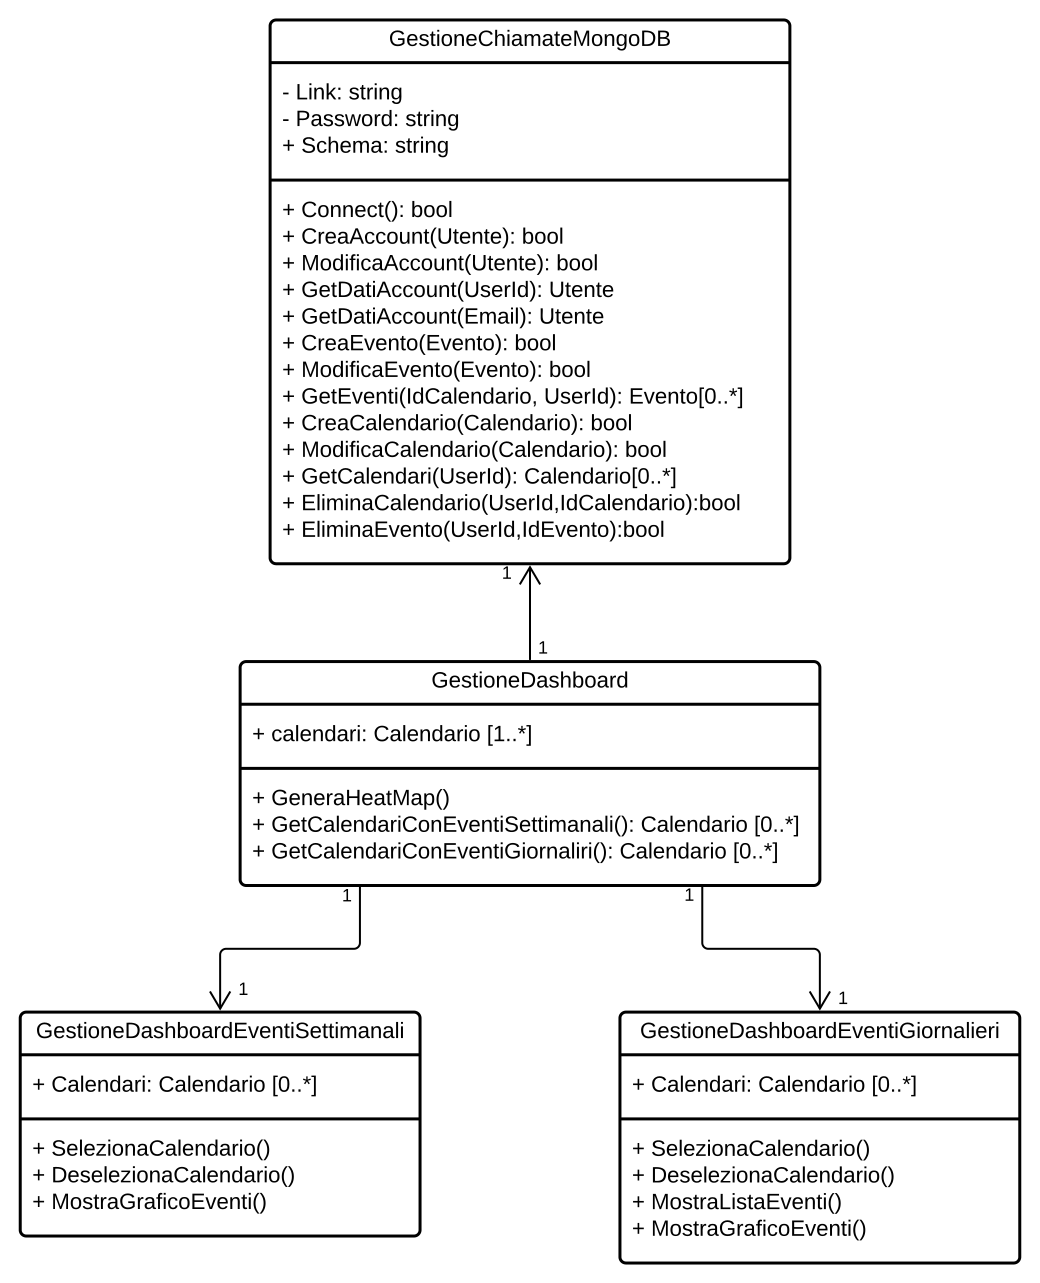
\includegraphics[width=1\textwidth]{img/FrontEnd/Dashboard/Dashboard.png}
    \end{center}
    
    \begin{listaPersonale2}{FE}
        \elemento[ATTIVITA' SVOLTE QUESTA SETTIMANA] {fe:3.1} Nella sezione “Attività svolte questa settimana” viene mostrato un grafico a barre delle varie attività svolte per ogni giorno della settimana (RF9), l’altezza delle barre corrisponde al quantitativo di ore dedicate a quell’attività.

        \begin{center}
            \includegraphics[width=0.53\textwidth,height=0.18\textheight]{img/FrontEnd/Dashboard/graficoBarre.png} %questa vorrei che fosse una wrap figure
        \end{center}
        
        \elemento[SITUAZIONE SCADENZA ATTIVITA'] {fe:3.2} Nella sezione “Situazione scadenze attività” è presente in basso una heatmap riguardo al tempo che deve essere dedicato ogni giorno per rispettare le varie deadline(RF9). La legenda sopra la heatmap mostra che più è tendente il colore al rosso, più ore devono essere impiegate nello specifico periodo di tempo.
        \begin{center}
            \includegraphics[width=0.45\textwidth,height=0.18\textheight]{img/FrontEnd/Dashboard/heatMap.png} %questa vorrei che fosse una wrap figure
        \end{center}
        
        \elemento [ATTIVITA’ SVOLTE OGGI e GRAFICO ATTIVITA' SVOLTE] {fe:3.3} Nella sezione “Attività svolte oggi” è presente una lista delle attività della giornate, da cui si possono ottenere anche le varie sottoattività. 
        La sezione “Attività svolte oggi” è sincronizzata con il grafico a torta presente nel “Grafico attività svolte” (RF9). Il grafico presenta le attività presenti in “Attività svolte oggi” con una dimensione proporzionata al tempo da spendere.
        \begin{center}
            \includegraphics[width=0.72\textwidth,height=0.2\textheight]{img/FrontEnd/Dashboard/selezionatoAttività.png} 
        \end{center}
        \begin{center}
            \includegraphics[width=0.72\textwidth,height=0.2\textheight]{img/FrontEnd/Dashboard/Dashboard3.png} %bisogna un modo per mettere queste due immagini bene, perché in colonna non so quanto mi piacciano
        \end{center}          
    \end{listaPersonale2}
    
    \elemento [SCHERMATA ATTIVITA'] {fe:4} Nella schermata attività è presente una tabella delle attività della giornata con le varie informazioni, ovvero: titolo, descrizione, categoria, priorità, durata (RF5), posizione (RF8.2). Inoltre ci sono dei tasti con cui si può rimandare e ritardare l’attività (RF10) e, infine, un tasto per indicare di averla completata. A fine giornata di default tutti gli impegni sono posti come completati; per modificare tale opzione deve intervenire l’utente.
    
    \elemento [SCHERMATA EVENTI] {fe:5} Nella schermata eventi sono presenti tutti i comandi che riguardano la compilazione, modifica degli eventi (RF5) , creazione di un calendario (RF 2.2.2), creazione di raggruppamento di attività ed eliminazione di un evento (RF5).
    Nella sezione sottostante, è presente una lista dei vari calendari e raggruppamenti, che selezionati una alla volta aprono i rispettivi form di modifica e creazione, dove sono presenti tutti i campi citati in RF5 per l’aggiunta e modifica di impegni, RF13 per modifica e aggiunta di calendario. 
    %qua dipende dalla formattazione andrebbe un clearpage
    \begin{figure}[H]
        \centering
        \includegraphics[width=1\textwidth]{img/FrontEnd/Eventi/SottoAttività.png}
        \caption{schermata quando si apre la schermata "Eventi"}
    \end{figure}
    \begin{figure}[h]
        \centering
        \includegraphics[width=1\textwidth]{img/FrontEnd/Eventi/Calendario/CreaCalendario.png}
        \caption{schermata quando si seleziona uno dei comandi}
    \end{figure}
    \begin{listaPersonale2}{FE}
        
        \elemento[SCHERMATA CREA/MODIFICA EVENTO] {fe:5.1}

        \begin{center} 
            \begin{figure}[H]
            \centering\includegraphics[width=0.49\textwidth,height=0.35\textheight]{img/FrontEnd/Eventi/Evento/CreaEvento.png}
            \centering\includegraphics[width=0.49\textwidth,height=0.35\textheight]{img/FrontEnd/Eventi/Evento/ModificaEvento.png}
            \end{figure}
        \end{center}

        
        \elemento[SCHERMATA CREA/MODIFICA RAGGRUPPAMENTO] {fe:5.2}

        \begin{center} 
            \begin{figure}[H]
            \centering\includegraphics[width=0.49\textwidth,height=0.35\textheight]{img/FrontEnd/Eventi/Raggruppamento/CreaRaggruppamento.png}
            \centering\includegraphics[width=0.49\textwidth,height=0.35\textheight]{img/FrontEnd/Eventi/Raggruppamento/ModificaRaggruppamento.png}
            \end{figure}
        \end{center}
        
        \elemento[SCHERMATA CREA/MODIFICA CALENDARIO] {fe:5.3}

        \begin{center} 
            \begin{figure}[H]
            \centering\includegraphics[width=0.49\textwidth,height=0.35\textheight]{img/FrontEnd/Eventi/Calendario/CreaCalendario1.png}
            \centering\includegraphics[width=0.49\textwidth,height=0.35\textheight]{img/FrontEnd/Eventi/Calendario/ModificaCalendario.png}
            \end{figure}
        \end{center}
        
    \end{listaPersonale2}
    
    \elemento [SCHERMATA ABITUDINI] {fe:6} Nella schermata “Abitudini”, l’utente può visualizzare la lista delle abitudini del proprio calendario. Inoltre c’è la possibilità di aggiungere, modificare ed eliminare (RF5) le abitudini del proprio calendario, ovvero le attività ripetute in un periodo determinato di tempo (RF5, 5.5), grazie alla sezione che si trova alla destra, dove si apre un form quando si va ad aggiungere e modificare un’ abitudine.
    \begin{center}
        \includegraphics[width=1\textwidth]{img/FrontEnd/Abitudini/Abitudini.png}
    \end{center}

    \elemento [SCHERMATA ROUTINE] {fe:7} Nella schermata “Routine” l’utente ha possibilità di visualizzare e gestire tutte le proprie routine, ovvero attività che ripete tutti i giorni (RF5,5.5), come dormire, mangiare e lavorare. L’utente ha la possibilità di definire quante ore e quando avere queste attività di routine, oppure lasciare al sistema di definire da solo quando avere quell’evento seguendo le regole definite in RF6.
    

    


\end{listaPersonale}


(Inoltre i cookie saranno usati per mantenere l'accesso così da evitare di fare il login ogni volta che si vuole utilizzare la piattaforma.)
\section{Requisiti Back-End}
\label{sec:RequisitiBackEnd}

Servizi usati
\begin{itemize}
    \item Google Maps / OpenStreetMaps
    \item Google Calendar
    \item PayPal/Stripe
    \item Auth0
    \item Cloudflare
\end{itemize}

\ref{rnf:4.3} (Si può adottare una programmazione a microservizi in modo tale da far si che se c'è un problema su un mezzoservizio il resto del sito continua a funzionare correttamente)

\end{document}
